%% This is the Chapter 3

%\begin{hyphenrules}{nohyphenation}
\chapter{AN R PACKAGE FOR STUDYING EVOLUTIONARY INTEGRATION AMONG SEVERAL TRAITS ON PHYLOGENETIC TREES}
%\end{hyphenrules}

\section{Abstract}

Evolutionary integration occurs when two or more phenotypes evolve in a correlated fashion. Correlated evolution among traits can happen due to genetic constraints, ontogeny, and selection and have an important impact on the trajectory of phenotypic evolution. Phylogenetic trees can be used to study such pattern on macroevolutionary time scales by estimating the strength of evolutionary covariance among traits through time and across clades. However, only few applications implement models to conduct comparative analyses of evolutionary integration. We introduce a Bayesian Markov chain Monte Carlo approach to estimate the evolutionary correlation among two or more traits using the evolutionary rate matrix ($\mathbf{R}$). $\mathbf{R}$ is a covariance matrix that represents both the rates of evolution of each trait and the structure of evolutionary correlation among traits. Here we present the R package \texttt{ratematrix}, a resource to test hypotheses of evolutionary integration using multivariate data and phylogenetic trees. \texttt{ratematrix} provides a flexible framework allowing for any number of evolutionary rate matrix regimes fitted to the same phylogenetic tree and it incorporates the uncertainty associated with parameter estimates, ancestral state reconstruction and phylogenetic estimation in the analyses. The \texttt{ratematrix} package uses a novel pruning algorithm that significantly improve computational time. We also provide specific functions that facilitate users to conduct long MCMC analysis when computational resources are limited.

\section{Introduction}

Evolutionary changes in one trait are often associated with changes in other traits, such that species traits often do not vary independently of each other \citep{Olson_Miller_1958}. This pattern can be observed in the covariation among traits both within and among populations \citep{arnold_constraints_1992, arnold_adaptive_2001, revell_testing_2008, revell_phylogenetic_2009}. The pattern of correlated evolutionary changes among two or more traits is known as evolutionary integration and can be a result of genetic constraints (e.g., pleiotropy), ontogenetic integration, or correlated selection \citep{arnold_constraints_1992, arnold_adaptive_2001, pigliucci_evolvability_2004, goswami_fossil_2015, melo_modularity:_2016}. Although evolutionary integration is ubiquitous across the tree of life, only few comparative methods and associated software applications to date implement models that can estimate evolutionary correlations among traits using phylogenetic trees \citep{revell_testing_2008, hohenlohe_mipod:_2008, revell_phylogenetic_2009, bartoszek_phylogenetic_2012, adams_geomorph:_2013, Clavel_mvmorph, goolsby_rphylopars:_2016}. 

Here we describe the R package \texttt{ratematrix}, which implements a Bayesian estimate of evolutionary rate matrices \citep[ $\mathbf{R}$;][]{revell_testing_2008} fitted to phylogenetic trees and trait data using Markov chain Monte Carlo \citep[as described in][]{caetano_sysbio_2017}. The $\mathbf{R}$ matrix is a variance-covariance matrix that describes the rates of trait evolution under Brownian motion in the diagonals and the evolutionary covariance among traits (i.e., the pattern of evolutionary integration) in the off-diagonals \citep{revell_testing_2008, revell_phylogenetic_2009, adams_assessing_2014}. With such a matrix we are able to simultaneously investigate the pace of evolution and the structure of evolutionary integration among two or more continuous traits evolving along the branches of a phylogenetic tree. We can also fit multiple $\mathbf{R}$ matrices to the same tree in order to test hypothesis of shifts in the evolutionary integration of these traits across clades on the tree. 

The $\mathbf{R}$ matrix can be estimated using current R packages, however all available implementations rely on point estimates using maximum likelihood. In contrast, the use of a Bayesian framework, as presented here, allows for direct incorporation of uncertainty in parameter estimates in the form of a posterior distribution \citep{caetano_sysbio_2017}. This is especially important because covariances can be hard to estimate when the number of observations is small relative to the number of parameters in the model, which is commonplace among phylogenetic comparative studies in general.

\section{ The model and MCMC implementation }

To study the pattern of correlated evolution among two or more continuous traits we use the model described by \citet{revell_testing_2008}, which consists of a multivariate Brownian motion model with rate equal to the $\mathbf{R}$ matrix and root value equal to the vector $\mathbf{a}$ \citep[see Equations 2 and 3 in][]{revell_phylogenetic_2009}. Our implementation allows for multiple independent rate regimes fitted to different branches of the phylogenetic tree \citep[as in][]{revell_phylogenetic_2009}. Rate regimes can be either fixed \textit{a priori} or a collection of multiple regime configurations can be included in the analysis. For example, multiple regimes applied to the same analysis could be samples from a stochastic character mapping \citep{huelsenbeck_stochastic_2003}, alternative reconstructions due to missing data, or other plausible hypotheses. However, all regimes need to share the same data at the tips of the tree and same number of rate matrices fitted to the tree. The \texttt{ratematrix} package implements Metropolis-Hastings Markov chain Monte Carlo (MCMC) to estimate the posterior distribution of each $\mathbf{R}$ matrix fitted to the tree and the vector of phylogenetic root values ($\mathbf{a}$).

Here we detail the proposal distribution used for each set of parameters as well as the options of prior densities currently implemented in the package. At each step of the MCMC chain we choose between the vector of root values and the set of one or more $\mathbf{R}$ matrices by drawing from a binomial distribution. The probability that each of these two sets of parameters will be updated is fixed throughout the chain, but can be determined by the user (see function \texttt{ratematrixMCMC}). Every time that the set of rate matrices is chosen, only one $\mathbf{R}$ matrix is updated but all $\mathbf{R}$ matrices fitted to the tree are equally likely to be updated. In contrast, once chosen, the root value for every trait is updated simultaneously. Updates are performed with different configurations of sliding window proposal distributions.

We implemented a uniform distribution with width controlled by the parameter \texttt{`w\_mu'} as the proposal distribution for each element of the vector of phylogenetic means. In contrast, the proposal of $\mathbf{R}$ matrices requires a more elaborate scheme, since variance-covariance matrices are constrained to be positive definite. Furthermore, $\mathbf{R}$ matrices describe both the rate of evolution of the traits and their pattern of evolutionary correlation, so the proposal distribution needs to provide good mixing for both the variance of each trait and the correlation structure of such matrices. We implemented a separation strategy \citep{barnard_modeling_2000, zhang_sampling_2006, liu_comparison_2016} proposal scheme which consists of making updates to the vector of standard deviations and the correlation matrix derived from the variance-covariance matrix in separate steps (Figure \ref{fig:proposal}). The vector of standard deviations can be updated directly using a sliding window proposal distribution. On the other hand, the proposal scheme for the correlation matrix requires two steps: first, draw covariance matrices from an inverse-Wishart distribution; and second, we derive correlation matrices from this sample. Finally, we recompose the evolutionary rate matrix in order to calculate the likelihood of the model. Figure \ref{fig:proposal} shows a diagram that describes the procedure. Note that the vector of standard deviations generated by decomposing the variance-covariance matrix is not evaluated by the likelihood of the model \citep{zhang_sampling_2006}. As a result of this parameter-extension approach, we need to correct the acceptance ratio for the transformation from variance-covariance matrix to the corresponding correlation matrix and vector of variances (Figure \ref{fig:proposal}). This proposal scheme allows for independent priors and proposals for the rates of evolution and the evolutionary integration among traits. The \texttt{ratematrix} package allows control over the width of the uniform sliding window proposal for the vector of standard deviations (`\texttt{w\_sd}') as well as the degrees of freedom of the inverse-Wishart (`\texttt{v}') used to sample correlation matrices.

\pagebreak

The prior densities for the model naturally follow the proposal scheme implemented. Prior densities are determined for the vector of root values, the vector of standard deviations and the correlation matrix (which is sampled by a transformation from the inverse-Wishart distribution). The separation between standard deviations and correlation matrix enable users to translate their biological intuition about the pace and mode of evolution into model parameters in a straightforward manner. The user can set independent priors (options are uniform, normal or log-normal) for both the vector of root values and the vector of standard deviations of the $\mathbf{R}$ matrices. For the correlation matrix that, together with the standard deviation, will constitute the $\mathbf{R}$ matrix the user can set the degrees of freedom ($\nu$) and the scale matrix ($\Psi$) of the inverse-Wishart distribution. Small values for $\nu$ make the distribution wider (Figure \ref{fig:prior_samples}, top) whereas larger values reduce the variance of the distribution, so samples will be closer to $\Psi$ and, as a result, the prior will be more informative (Figure \ref{fig:prior_samples}, bottom). Note from Figure \ref{fig:prior_samples} that a change in the parameters of the inverse-Wishart prior on the correlation matrix will not change the prior distribution of variances. Since the inverse-Wishart will only be used to sample correlation matrices, $\Psi$ can be set as any correlation matrix or variance-covariance matrix.

\section{ Description of the \texttt{ratematrix} R package }

The package \texttt{ratematrix} offers a plethora of functions to allow flexible choices of prior distributions for all parameters in the model, customizable MCMC chains, plots, and robust analyses of convergence (Table \ref{tab:functions}). The package can be installed from our \texttt{github} repository using the R package \texttt{devtools}:\\
\\
\hspace*{20pt} \texttt{ devtools::install\_github("Caetanods/ratematrix", build\_vignettes = TRUE) }
\hspace*{20pt} \texttt{ library(ratematrix) }\\
\\
The option \texttt{build\_vignettes} will make the package vignettes available after installation. A list of vignettes can be accessed using:\\
\\
\hspace*{20pt} \texttt{ browseVignettes("ratematrix") }\\
\\
We will use the same data from \citet{caetano_sysbio_2017} on mainland and island anole lizards as a demonstration of the package. In this study we test whether the radiation of anole lizards from Central and South America to the Caribbean islands was associated with a shift in the pattern of evolutionary integration among morphological traits (head length, tail length and snout-vent length). Here the phylogenetic tree (object \texttt{anoles\$phy}) is a stochastic map with two regimes produced with the package \texttt{phytools}, one rate regime for island and other for mainland species (see Figure \ref{fig:anoles_simmap}). Both the trait data and phylogenetic tree are included in the \texttt{ratematrix} package.\\
\\
\hspace*{20pt} \texttt{ data(anoles) \# Load trait data and phylogeny.}

\subsection{ Estimating rates of correlated evolution }

After loading the package and data, we choose the prior distributions for the MCMC chain. We set a uniform prior for the vector of root values and variances and a marginally uniform prior for the covariance matrices, following \citet{barnard_modeling_2000} (see also documentation for \texttt{makePrior}). The marginally uniform prior produces uniform distributions for each of the covariance terms ($\sigma_{i,j}^{2}$ for $i \neq j$) of the variance-covariance matrix after integrating over the uncertainty of the other parameters (i.e., the marginal distribution for $\sigma_{i,j}^{2}$). Many characteristics of the Markov chain Monte Carlo can be customized (see documentation for \texttt{ratematrixMCMC}). We encourage users to run short preliminary chains in order to adjust the width of the proposal distributions for each set of parameters in function of the acceptance ratio (see function \texttt{logAnalyzer}) prior to a full MCMC chain analysis. This procedure can improve the mixing of the chains, which might decrease the number of generations required until convergence and increase the effective sample size (ESS) of the posterior distribution. The following lines of code will run only a short example, starting with a random sample from the prior distribution. The package also provide results from previous MCMC analyses with this same data as examples.\\
\\
\hspace*{20pt} \texttt{ estimateTimeMCMC(data=anoles\$data[,1:3], phy=anoles\$phy, gen=10000) }\\
\hspace*{20pt} \texttt{ handle <- ratematrixMCMC(data=anoles\$data[,1:3], phy=anoles\$phy \newline, prior="uniform", gen=10000)}\\
\\
The \texttt{estimateTimeMCMC} function estimates the time for the MCMC chain whereas \linebreak \texttt{ratematrixMCMC} runs it. The MCMC function writes one file with the parameter samples and another with the log information for each generation. Both files are marked with a unique identifier that prevents multiple chains of overwriting each other. The \texttt{handle} object is a list containing detailed information about the MCMC chain and is required in order to read the posterior distribution from files, analyze the log information and continue an unfinished MCMC chain. Bellow we show an example of how to read the posterior distribution from the files. Then, we make plots (Figure \ref{fig:anolesGrid}) and calculate summary statistics based on results of a converged MCMC chain provided as example data.\\
\\
\hspace*{20pt} \texttt{ ( short\_chain <- readMCMC(handle, burn=0.25, thin=1) ) } \\
\hspace*{20pt} \texttt{ logAnalyzer(handle, burn=0.25, thin=1) \# Log information for the chain.}\\
\hspace*{20pt} \texttt{ plotRatematrix(chain=short\_chain) \# Plots the short chain. } \\
\hspace*{20pt} \texttt{ plotRootValue(chain=short\_chain) \# Plots the short chain. } \\
\\
\hspace*{20pt} \texttt{ data(anolesPost) \# Load example of posterior distribution.} \\
\hspace*{20pt} \texttt{ plotRatematrix(chain=anolesPost\$chain1) } \\
\hspace*{20pt} \texttt{ plotRootValue(chain=anolesPost\$chain1) } \\
\hspace*{20pt} \texttt{ checkConvergence(anolesPost\$chain1, anolesPost\$chain2) } \\
\hspace*{20pt} \texttt{ testRatematrix(chain=anolesPost\$chain1, par="correlation") } \\
\hspace*{20pt} \texttt{ testRatematrix(chain=anolesPost\$chain1, par="rates") }\\
\\
The \texttt{logAnalyzer} function calculates the acceptance ratio for each parameter of the model and plots the trace of the log-likelihood for the MCMC chain. The plot functions show the posterior distribution of parameter estimates. \texttt{plotRatematrix} produces a plate with histograms for the rate of evolution of each trait (diagonal) and the pairwise evolutionary covariation among traits (upper-diagonal). The lower-diagonal plots show ellipses for the 95\% confidence interval of the bivariate distribution between each pair of traits. Different from the histograms, the ellipses are only a sample from the posterior distribution (see documentation for \texttt{plotRatematrix}).

Here we applied the test of convergence for the chains using \citet{gelman_R_1992} potential scale factor analysis (see function \texttt{checkConvergence}). This convergence test requires two or more independent MCMC chains and compares the variance of parameter estimates between chains and within each chain.

The \texttt{testRatematrix} function calculates a series of summary statistics based on the pairwise degree of overlap among the posterior distribution of $\mathbf{R}$ matrices fitted to same phylogenetic tree \citep{caetano_sysbio_2017}. If this overlap exceeds 5\%, then we can conclude that the difference between posterior parameter estimates is not strong enough to support the hypothesis that regimes are representations of distinct macroevolutionary patterns. When we compare the posterior distribution for the evolutionary correlation (\texttt{par="correlation"}; overlap of 0.4) and the rates of evolution for each trait (\texttt{par="rates"}; overlap of 0.0002) there is no evidence for a shift in the pattern of evolutionary integration but island anole lineages show faster rates of trait evolution when compared to mainland lineages \citep[Figure \ref{fig:anolesGrid}, see also][]{caetano_sysbio_2017}. We refer readers to \citet{caetano_sysbio_2017} for an extensive simulation study of the performance of the method as well as the use of summary statistics under a diverse set of scenarios of correlated evolution.

\subsection{ Integration of uncertainty in regime configurations }

One of the advantages of Bayesian implementations is that analyses can integrate uncertainty from different sources. Rate regimes, for example, are used to map the set of nodes and branch lengths that will be assigned to each $\mathbf{R}$ matrix fitted to a phylogenetic tree. Such regimes are usually determined \textit{a priori} by ancestral estimate, since we often are interested in the association between some characteristic and a possible shift in the pattern of evolutionary integration among traits. However, ancestral state estimates can be uncertain and alternative reconstructions are often possible, specially when the states of the characteristics under study are polymorphic or of dubious interpretation. Nevertheless, most comparative methods are implemented to estimate the parameters of the model with a single regime configuration and users need to perform multiple independent analyses in order to incorporate uncertainty associated with ancestral state estimates.

The package \texttt{ratematrix} offers a different approach by allowing a pool of phylogenetic trees to be directly incorporated in the MCMC. This pool can comprise repeated simulations from a stochastic mapping analysis, equally parsimonious ancestral state reconstructions or even a random sample of trees from the posterior distribution of a phylogenetic inference analysis. In order to incorporate the pool of trees, we randomly sample one phylogenetic tree each time the likelihood function of the model is evaluated. Note that this procedure is not the same as a joint Bayesian MCMC estimate of the trait model and the phylogenetic tree because the posterior distribution of rate regimes or phylogenetic trees is not sampled as part of the MCMC. However, the posterior distribution of parameter estimates for the model is sampled conditioned on the pool of trees provided by the user. Bellow we show how to create an analysis based on a pool of stochastic mapping simulations:\\
\\
\hspace*{20pt} \texttt{ library(phytools)  \# Using \citet{revell_phytools:_2012}. } \\
\hspace*{20pt} \texttt{ state <- setNames(anoles\$data\$Location, rownames(anoles\$data)) } \\
\hspace*{20pt} \texttt{ phy\_map <- make.simmap(anoles\$phy, x=state, nsim=100) } \\
\hspace*{20pt} \texttt{ handle\_map <- ratematrixMCMC(data=anoles\$data[,1:3], phy=phy\_map \newline , prior="uniform", gen=10000, outname="phy.pool") } \\
\hspace*{20pt} \texttt{ logAnalyzer(handle\_map, burn=0.25, thin=1) }\\

\pagebreak

When a pool of phylogenetic trees is provided for the MCMC, \texttt{logAnalyzer} returns the acceptance ratio for each of the phylogenetic trees. Relative low acceptance ratio for a given tree means that proposals were rejected more often than with the rest of trees from the same pool. This might be due to a low likelihood score for the multivariate Brownian-motion model given the tree as a result of an unlikely topology, branch lengths or rate regime configuration. If this is the case, one can check if the tree has some particular attributes that make it distinct from other trees in the pool, since such patterns might carry important biological information. Furthermore, we recommend that an independent analysis is performed with such a tree (or trees) so that one can test whether results are significantly different than the former analysis using the entire pool.

\subsection{ Continuing unfinished chains or adding extra iterations }

The \texttt{ratematrix} package allows for continuing an unfinished MCMC analysis or to append additional generations to the previous MCMC chain. This is an essential feature given the computational burden associated with any Bayesian simulation approach. In both cases, the user needs to provide the \texttt{handle} object returned by the \texttt{ratematrixMCMC} function (or saved to the working directory). The following example will add iterations to the previous MCMC chain: \\
\\
\hspace*{20pt} \texttt{ handle\_map\_add <- continueMCMC(handle\_map, add.gen=1000) }\\
\\
One can use \texttt{continueMCMC} alongside \texttt{checkConvergence} to add generations to the MCMC until the chain(s) pass the convergence test. This is especially relevant given that the number of generations required for acceptable convergence is dependent on the data and the configuration of the sampler.

\section{ New pruning algorithm improves computational time }

The package \texttt{ratematrix} implements a novel algorithm to evaluate the likelihood function of a multivariate Brownian motion model when two or more $\mathbf{R}$ matrix regimes are fitted to the same phylogenetic tree \citep{caetano_sysbio_2017}. In previous implementations, a large matrix composed by the multiplication between the phylogenetic variance-covariance matrix, with dimension equal to the number of species in the tree, and the evolutionary rate matrix, with dimension equal to the number of traits, needed to be computed. However, any operation with such large matrices can become very computationally intensive. Recently, \citet{caetano_sysbio_2017} implemented an extension of \citet{felsenstein_1973} pruning algorithm that avoids such calculations. As a result, matrix operations need only to be performed with the evolutionary rate matrix ($\mathbf{R}$), which is usually a fairly small matrix. Figure \ref{fig:time_plot} shows the computational time for the likelihood function under different approaches. Computation using the full inverse and determinant of the matrices is the approach that scales worst with number of traits and size of the phylogeny. Although the `rpf' method \citep{Gustavson_rpf}, which avoids the computation of the full inverse and determinants, shows a significant improvement, the pruning algorithm has the best performance. With respect to the asymptotic upper bounds ($O$), all approaches scale equally with the number of traits in the analysis when the size of the phylogeny is held constant, but there is a remarkable improvement with the scaling in function of the number of tips in the phylogeny. The pruning algorithm scales with $O(n + r^{3})$ whereas the other methods scale with $O(n^{3} + r^{3})$, where $n$ is the number of tips in the phylogeny and $r$ is the number of traits. The reduction of time to evaluate the likelihood of the model is fundamental to the implementation of simulation based approaches such as the Bayesian Markov chain Monte Carlo estimates performed by the package \texttt{ratematrix} \citep{caetano_sysbio_2017}.

\section{ Resources }

\texttt{ratematrix} is an open-source R package that can be installed from the github repository \url{https://github.com/Caetanods/ratematrix}. A series of tutorials are available at \url{https://github.com/Caetanods/ratematrix/wiki}.

\pagebreak

\begin{table}[h]
\caption[Principal functions available in \texttt{ratematrix}.]{Principal functions available in \texttt{ratematrix}.}
\label{tab:functions}
\begin{center}
%% \begin{tabular}{cl}
\begin{tabularx}{\textwidth}{cX}
\hline 
Function & Description \\ 
\hline 
\texttt{checkConvergence}  & Perform tests of convergence with one or multiple MCMC chains. \\ 
\texttt{continueMCMC}  & Continue or add generations to a MCMC chain. \\
\texttt{estimateTimeMCMC}  & Estimate the time that a MCMC chain will take to run. \\
\texttt{likelihoodFunction}  & Compute the log-likelihood of the multivariate Brownian-motion model. \\
\texttt{logAnalyzer}  & Compute acceptance ratio for parameters and pool of phylogenies and make trace plots for the log-likelihood and acceptance ratio. \\
\texttt{makePrior} & Create prior densities for the model. \\
\texttt{makeStart} & Create starting point for the MCMC chain. \\
\texttt{mergePosterior} & Merge multiple chains from the same data into a single chain. \\
\texttt{mergeSimmap} & Merge rate regimes mapped to a phylogenetic tree. \\
\texttt{plotPrior} & Plot the prior distribution for the parameters of the model. \\
\texttt{plotRatematrix} & Plot the posterior distribution of evolutionary rate matrices ($\mathbf{R}$). \\  
\texttt{plotRootValue} & Plot the posterior distribution of root values (phylogenetic mean). \\
\texttt{ratematrixMCMC} & Make the Bayesian Markov chain Monte Carlo analysis. \\
\texttt{readMCMC} & Read MCMC samples from the \texttt{ratematrixMCMC} output file. \\
\texttt{samplePrior} & Draw samples from the prior density created by \texttt{makePrior}. \\
\texttt{simRatematrix} & Simulate data given a phylogenetic tree, evolutionary rate matrix and root values. \\
\texttt{testRatematrix} & Use summary statistics to test for shifts between rate regimes. \\
\hline
%% \end{tabular}
\end{tabularx} 
\end{center}
\end{table}

\pagebreak

\begin{figure}[h]
	\centering
	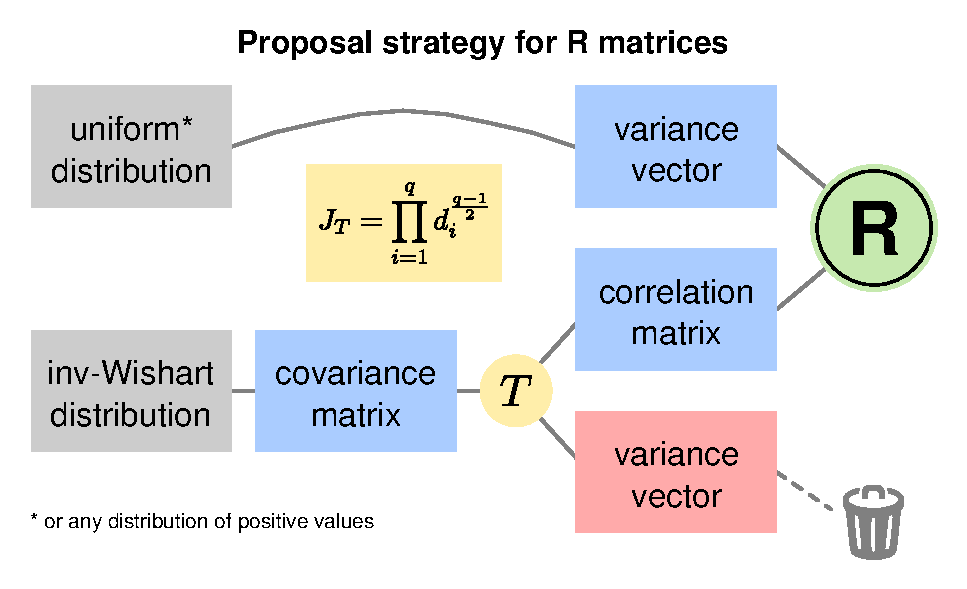
\includegraphics[scale=0.85]{separation_strategy_figure_updated}
	\caption[Diagram of the separation strategy proposal.]{Diagram of the separation strategy proposal \citep{barnard_modeling_2000}. Boxes in grey show the proposal distributions for the variance vector and correlation matrix that compose the evolutionary rate matrix ($\mathbf{R}$). Boxes in blue show the elements that are directly (or indirectly, in the case of the covariance matrix) evaluated in the acceptance step of the MCMC. The yellow circle shows the transformation ($T$) required to decompose the variance-covariance matrix sampled from a inverse-Wishart into a correlation matrix and the variance vector. The yellow square shows the formula for the Jacobian correction due to $T$ \citep{zhang_sampling_2006}, where $d_{i}$ stands for the variance of traits 1 to $q$. The red square demonstrates that a additional variance vector is produced in the process, but it is discarded. The green circle is a representation of the $\mathbf{R}$ matrix as a product between the variance vector and the correlation matrix.}
	\label{fig:proposal}
\end{figure}

\begin{figure}[h]
	\centering
	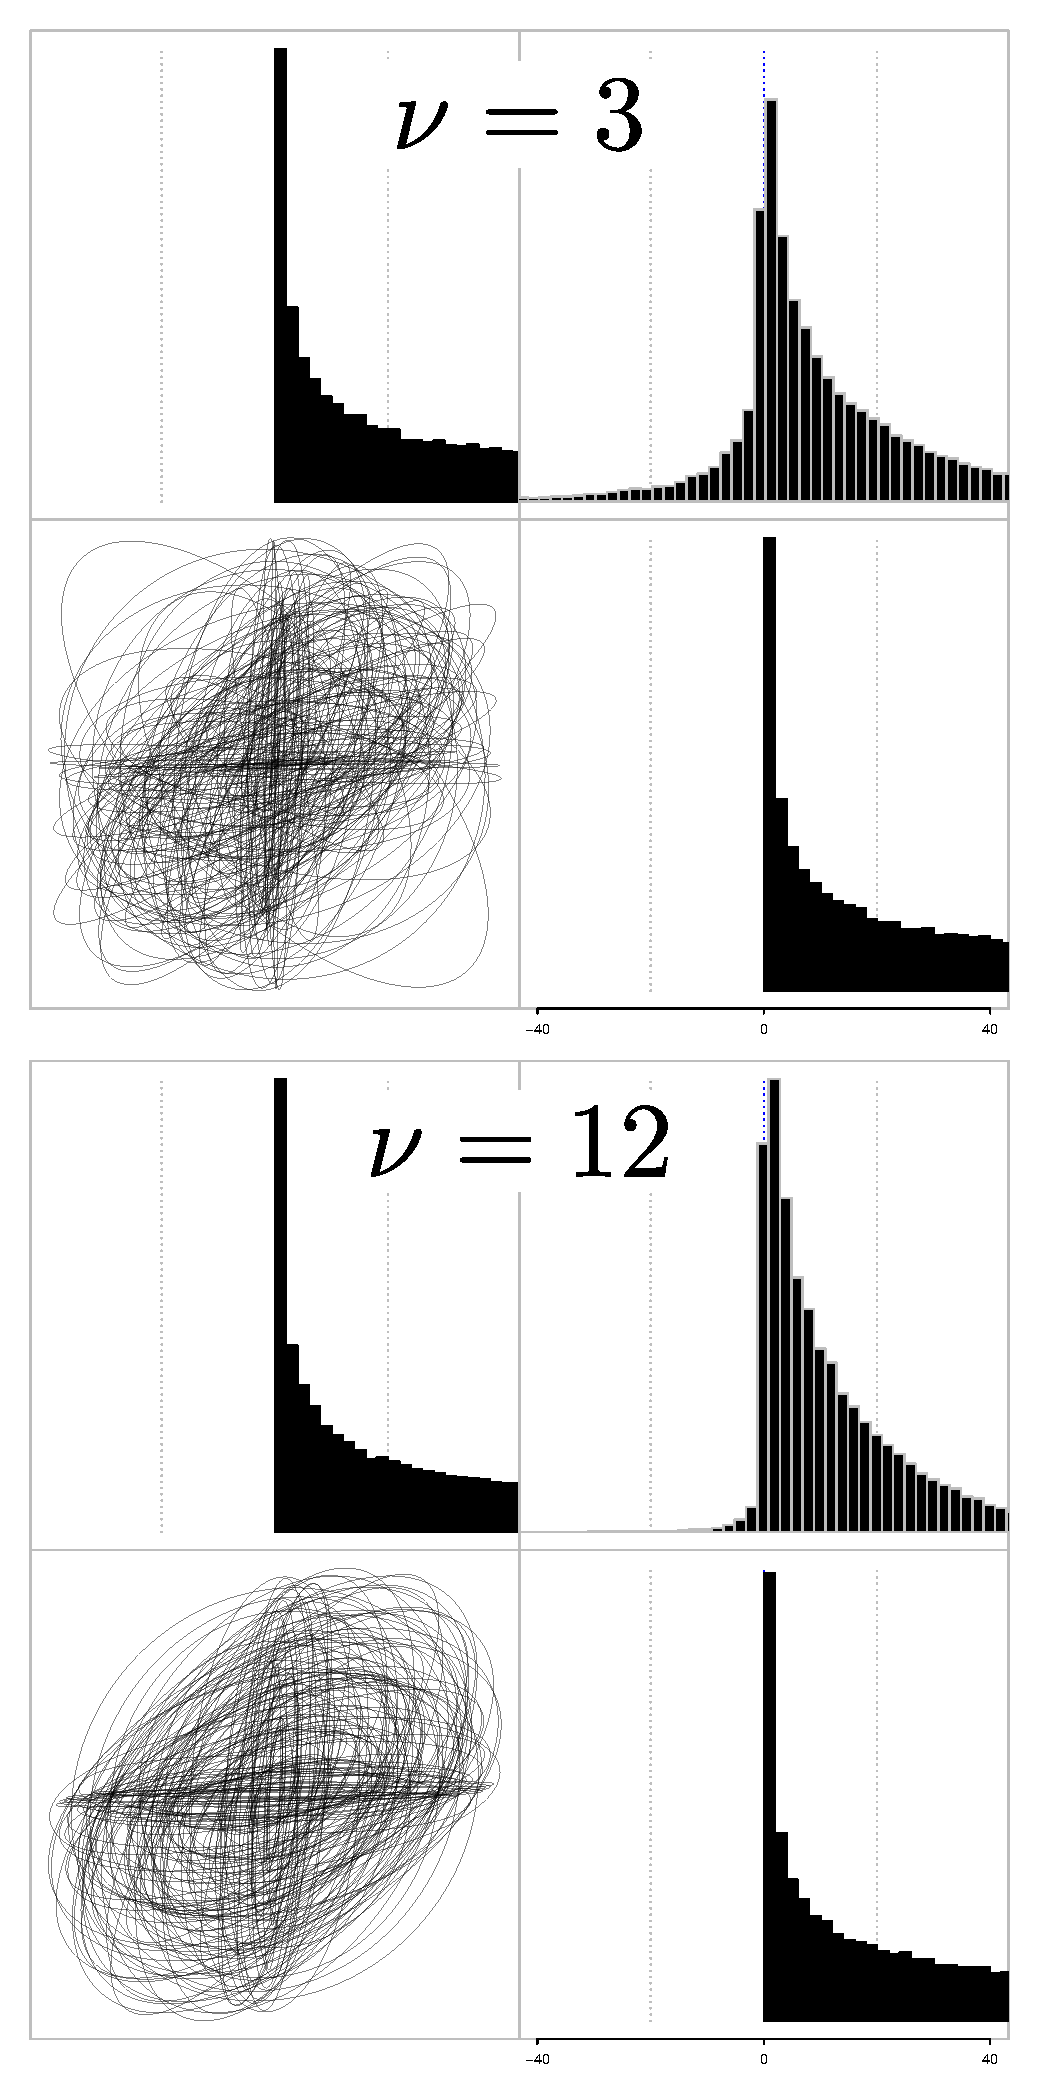
\includegraphics[scale=0.4]{weak_and_strong_prior}
	\caption[Samples from the prior of the evolutionary rate matrix ($\mathbf{R}$) for two simulated traits using the separation strategy.]{Samples from the prior of the evolutionary rate matrix ($\mathbf{R}$) for two simulated traits using the separation strategy \citep{barnard_modeling_2000}. Standard deviation was modelled as a uniform distribution between 0 and 10 and the correlation matrix was derived from a inverse-Wishart centered on a scale matrix with positive correlation (corr = 0.5). Top figure shows a weak prior with small value for the degrees of freedom parameter ($\nu$ = 3) whereas bottom figure are draws from a more informative prior ($\nu$ = 12). In each figure, the plots in the diagonal show evolutionary rates for each trait whereas the upper-diagonal plot shows the evolutionary covariation. Lower-diagonal plot show 150 randomly sampled ellipses representing the 95\% quantile for the bivariate distribution. Although both priors share the same scale matrix, when $\nu$ is small the prior distribution has more variance than when $\nu$ is larger. The diagonal plots are held constant since the prior distribution for the standard deviation is the same in both figures. Note that ellipses show both positive and negative correlation when the prior is weak (top figure) and positive or no correlation when the prior is more informative (bottom figure).}
	\label{fig:prior_samples}
\end{figure}

\begin{figure}[h]
	\centering
	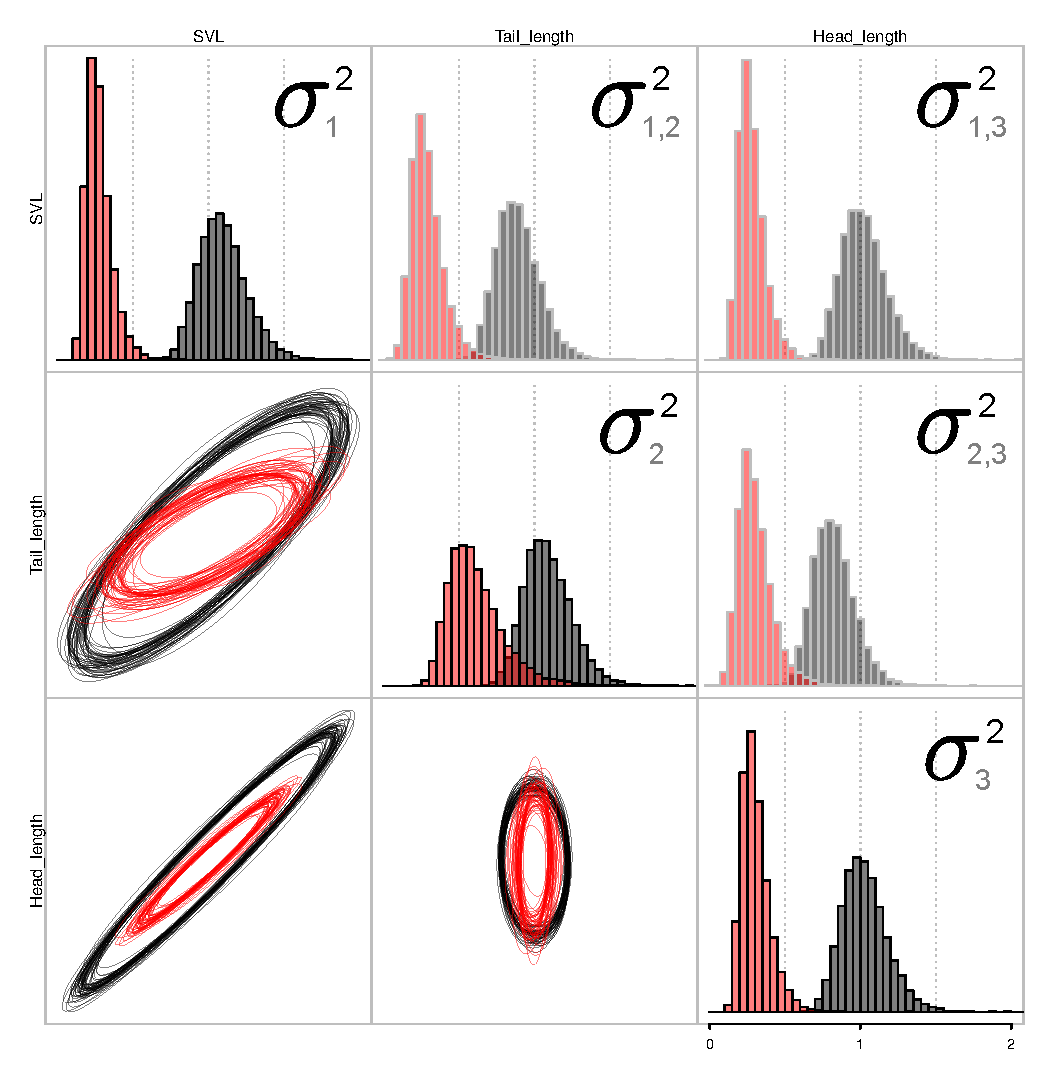
\includegraphics[scale=0.7]{ratematrix_plot_red_and_black_edited}
	\caption[Posterior distribution of the evolutionary rate matrix ($\mathbf{R}$) regimes fitted to the island anole and mainland anole lineages.]{Posterior distribution of the evolutionary rate matrix ($\mathbf{R}$) regimes fitted to the island anole (gray) and mainland anole (pink) lineages. A different $\mathbf{R}$ matrix were jointly estimated for each regime. The plots in the diagonal show evolutionary rates (variances) for each trait; $\sigma_{1}^{2}$ for SVL, $\sigma_{2}^{2}$ for tail length, and $\sigma_{3}^{2}$ for head length. Upper-diagonal plots show pairwise evolutionary covariation (covariances); $\sigma_{1,2}^{2}$ between SVL and tail length, $\sigma_{1,3}^{2}$ between SVL and head length, and $\sigma_{2,3}^{2}$ between tail length and head length. The ellipses in the lower-diagonal plots represent the 95\% confidence interval of each bivariate distribution for 50 randomly sampled $\mathbf{R}$ matrices from the posterior. The order of the ellipse plots is a mirror reflection from the upper-diagonal evolutionary covariance plots. Ellipses are only a sample of the posterior because a very large number of lines can become hard to visualize, however the user can set any number of samples (or the entire posterior).}
	\label{fig:anolesGrid}
\end{figure}

\begin{figure}[h]
	\centering
	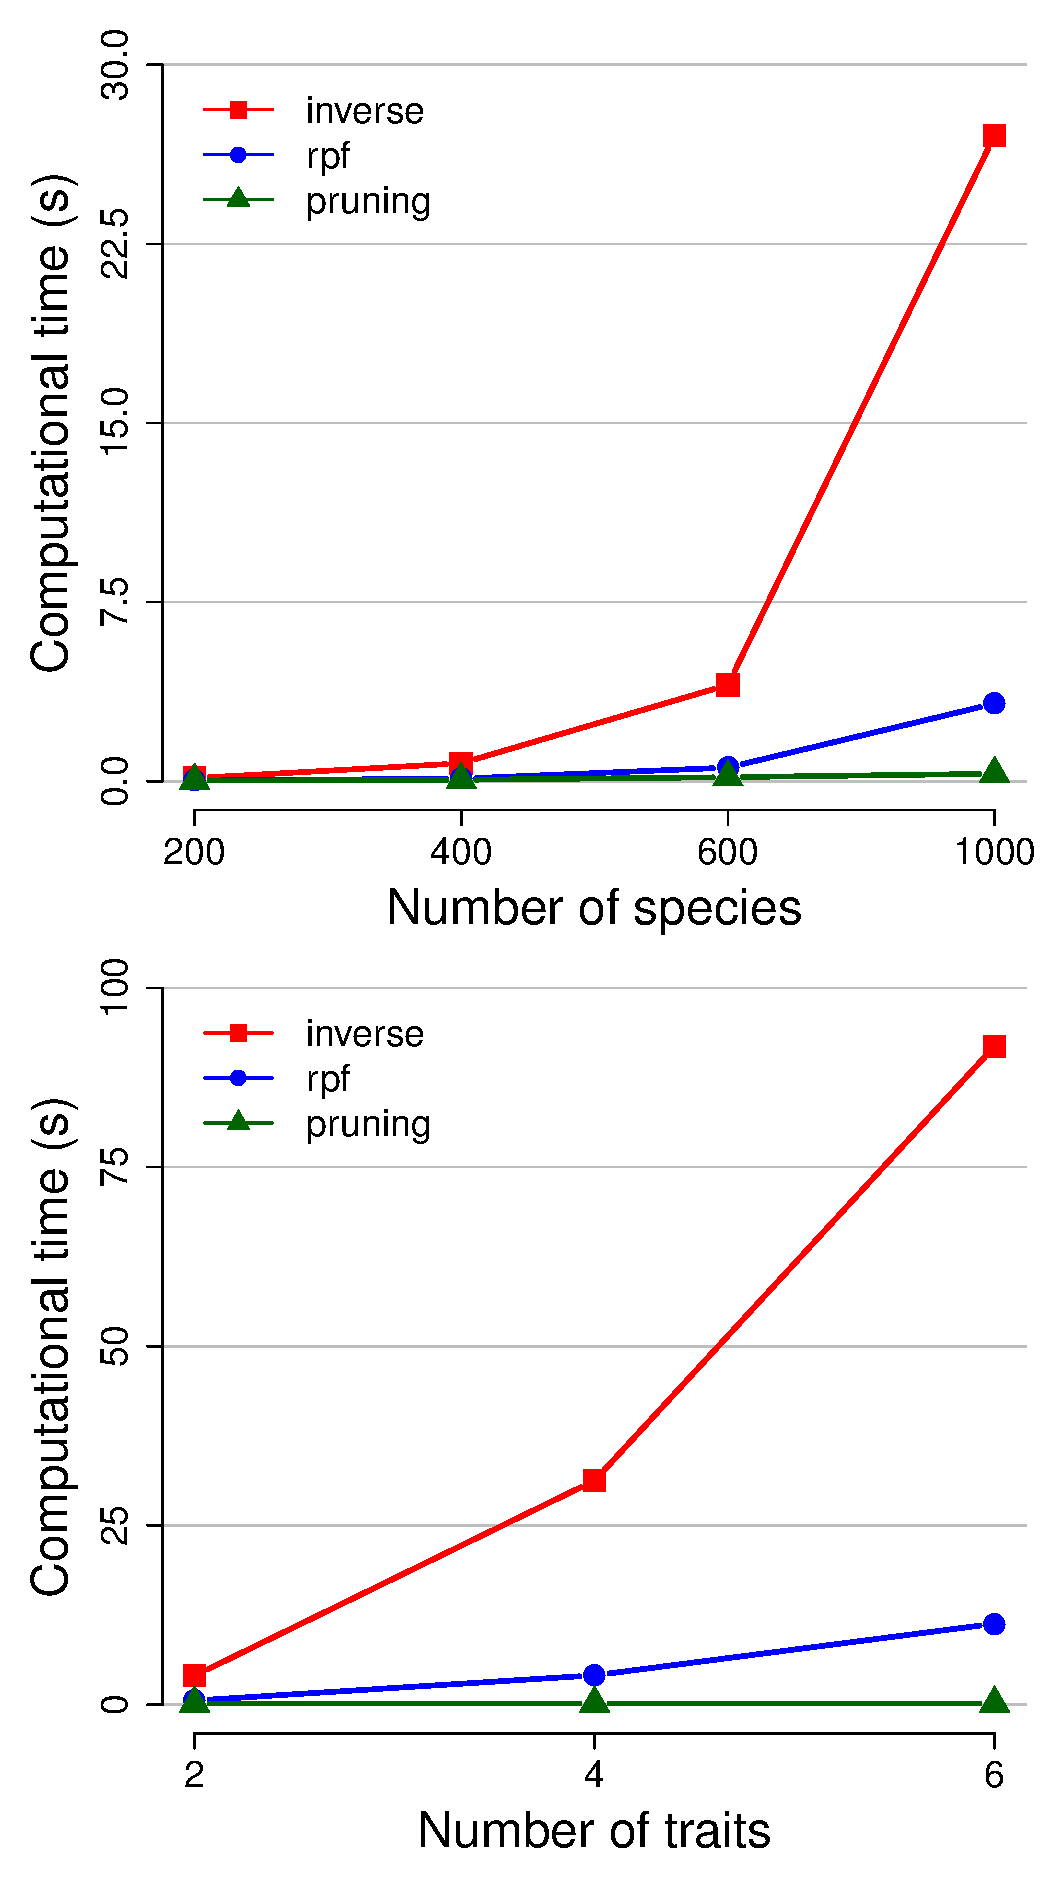
\includegraphics[scale=0.4]{time_plots}
	\caption[Time in seconds spent to compute the likelihood function using different approaches.]{Time in seconds spent to compute the likelihood function using different approaches. Top figure shows computational time for two traits and a phylogeny of different number of species. Bottom figure shows computational time with a phylogeny of 400 species and increasing number of traits. Both plots show a comparison among three approaches: `inverse' uses the full inverse and determinant of matrices as implemented in \texttt{phytools} \citep{revell_phytools:_2012}, `rpf' uses the rectangular full-packed format algorithm as implemented in \texttt{mvMORPH} \citep{Clavel_mvmorph}, and `pruning' uses \citet{felsenstein_1973} pruning algorithm as implemented in \texttt{ratematrix}.}
	\label{fig:time_plot}
\end{figure}

\begin{figure}[h]
	\centering
	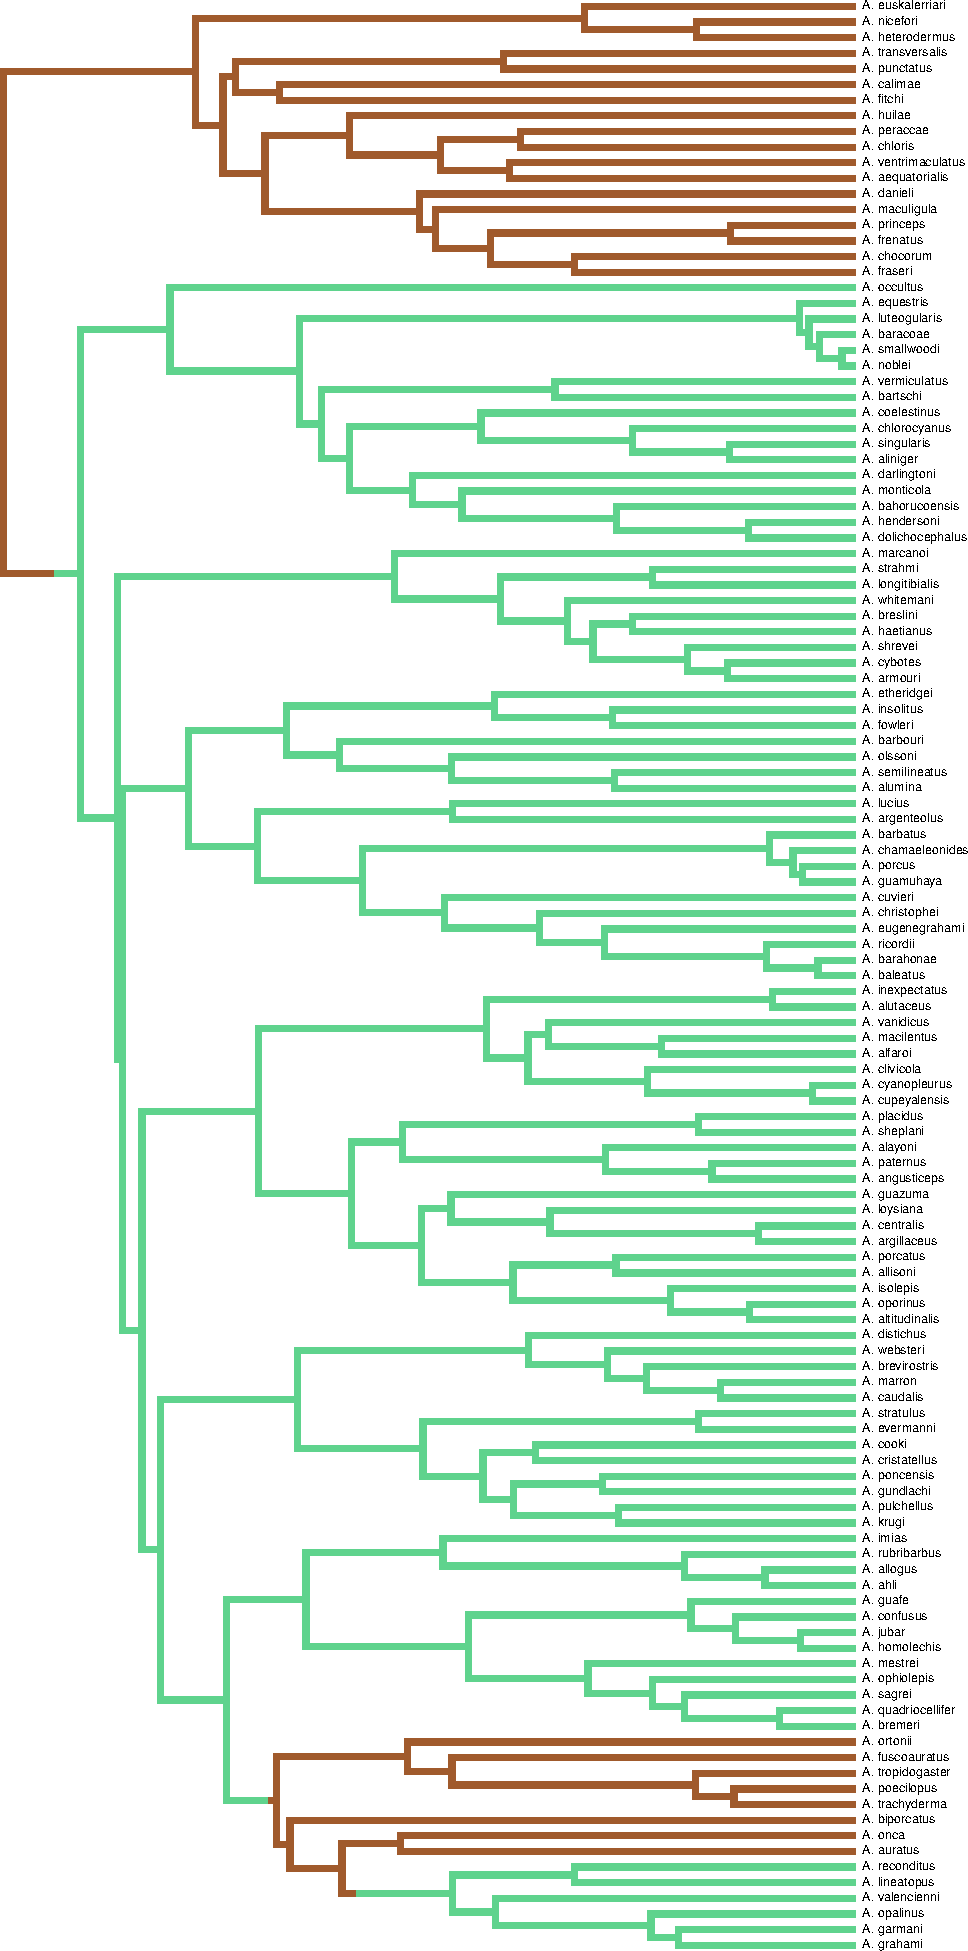
\includegraphics[scale=0.5]{anoles_simmap_tree}
	\caption[Maximum clade credibility phylogenetic tree for anole lizards made available by \citet{gamble_anolis_2014}.]{Maximum clade credibility phylogenetic tree for anole lizards made available by \citet{gamble_anolis_2014}. Only anole species included in the analysis are shown. Branches painted in brown represent mainland lineages whereas branches in green are island lineages. Regimes were mapped to the tree using stochastic mapping with root state set to mainland, as implemented in the package \texttt{phytools} \citep{revell_phytools:_2012}. Please refer to \citet{caetano_sysbio_2017} for more information.}
	\label{fig:anoles_simmap}
\end{figure}